\documentclass[12pt]{article}
\usepackage[margin=1in]{geometry}
\usepackage{graphicx}
\graphicspath{ {./} }


\title{Talkatiel Software Requirements and Planning}
\author{Brendan Byers, Ryan Sisco, Iliana J, Aidan Grimshaw}
\date{\today}

\begin{document}
\begin{center}
      \Large\textbf{Talkatiel Software Design Specification and User Interface}\\
      \large\textit{Brendan Byers, Ryan Sisco, Iliana Javier, Aidan Grimshaw, Yufei Zeng}\\
      \large{byersbr, siscor, javieri, grimshaa, zengyu}\\
   \end{center}

\section{User Interface Prototypes}
We have created three user interface prototypes to showcase the key user interactions that will make our app functional.

\subsection{Creating a New Post}
Users create a new post with a title and text content. When they press the submit button, a new post element is added to the database, with the attributes of title, text content, submission time, upvote/downvote count, and author as specified by the post class diagram.

\subsection{Auditing New Post}
Users view posts on the post viewing page of the app, which is the one that will be loaded when the app starts. Users will view posts sorted by the post sorting function, from which users can select a time range to view posts from, Ex: top posts from last 24 hours, week, month, year, or ever. Users will update the posts by pulling down on the top of the app, which will send a request to the server for the updated posts table, which will then be filtered by the post sorting function and displayed to the user in order of time.

\subsection{Viewing Page}
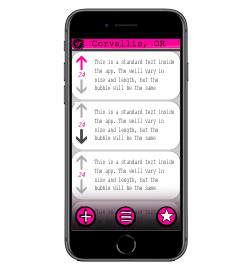
\includegraphics[scale=0.75]{img/homescreen}


\section{Class Diagram}
\section{Sequence Diagram}

\section{Meeting Report}

\subsection{Progress Made This Week}
\subsection{Plans for Next Week}
\subsection{Team Member Contributions}

\end{document}
